% Copyright 2005-2016 Airbus-EDF-IMACS-Phimeca
% Permission is granted to copy, distribute and/or modify this document
% under the terms of the GNU Free Documentation License, Version 1.2
% or any later version published by the Free Software Foundation;
% with no Invariant Sections, no Front-Cover Texts, and no Back-Cover
% Texts.  A copy of the license is included in the section entitled "GNU
% Free Documentation License".
\renewcommand{\filename}{docUC_CentralUncertainty_TaylorVarDecomposition.tex}
\renewcommand{\filetitle}{UC : Moments evaluation from the Taylor variance decomposition method and evaluation of the importance factors associated}

% \HeaderNNIILevel
% \HeaderIILevel
\HeaderIIILevel


\index{Taylor variance decomposition }
\index{Graph!Taylor variance decomposition  importance factors}
\index{Graph Manipulation!View}
\index{Graph Manipulation!Show}

The objective of this Use Case  is to evaluate the mean and standard deviation of the output variable of interest thanks to the Taylor variance decomposition method of order one or two.\\

Details on the  Taylor variance decomposition method may be found in the Reference Guide (\extref{ReferenceGuide}{see files Reference Guide - Step C -- Taylor variance decomposition / Perturbation Method}{stepC} and Step C' -- importance Factors derived from Taylor Variance Decomposition Method).\\




\requirements{
  \begin{description}
  \item[$\bullet$] the output variable of interest {\itshape output} of dimension $\geq 1$
  \item[$\bullet$] a RandomVector
  \end{description}
}
             {
               \begin{description}
               \item[$\bullet$] Mean and covariance of the variable of interest
               \item[type:] NumericalPoint, Matrix
               \item[$\bullet$] Importance factors from the Taylor variance decomposition method only for {\itshape output} of dimension 1
               \item[type:] NumericalPoint
               \end{description}
             }

             \textspace\\
             Python script for this UseCase :

             \inputscript{script_docUC_CentralUncertainty_TaylorVarDecomposition}

             \textspace\\

             Figure \ref{quadraticCumulImportanceFactors}  shows an importance factors pie evaluated from the Taylor variance decomposition method, in the beam example described in Eq.(\ref{equatPoutre}) before, where :
             \begin{itemize}
             \item $E$ follows the Beta($r = 0.94$, $t = 3.19$, $a = 2.78e7$, $b = 4.83e7$) distribution,
             \item $F$ follows the LogNormal($\mu = 3e5$, $\sigma = 9e3$, $\gamma = 1.5e4$)  distribution,
             \item $L$ follows the Uniform($a = 250$, $b=260$) distribution,
             \item $I$ follows the Beta($r = 2.5$, $t = 4.0$, $a = 3.1e2$, $b = 4.5e2$) distribution,
             \item the four components are independent.
             \end{itemize}



             \begin{figure}[H]
               \begin{center}
                 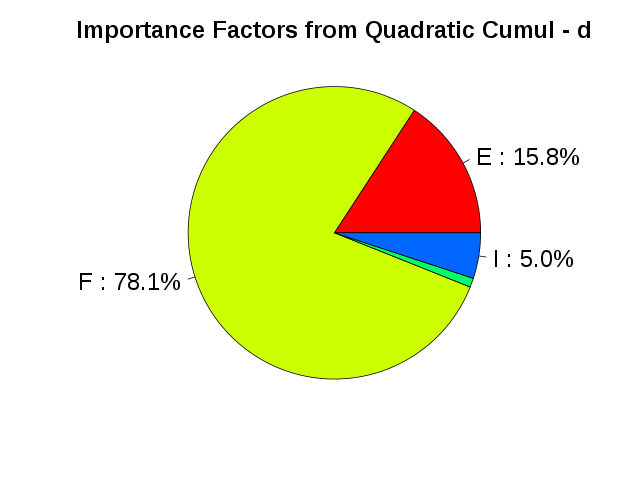
\includegraphics[width=10cm]{Figures/ImportanceFactorsDrawingQuadraticCumul.png}
               \end{center}
               \caption{Importance Factors from the Taylor variance decomposition method in the beam example.}
               \label{quadraticCumulImportanceFactors}
             \end{figure}
